\section{Materials and methods}

\subsection{Study design and inferential scope}

The study is an intensive analysis of one zebrafish fluorescence recording with
\VenueCohortBursts{} annotated spontaneous burst intervals. The canonical-v7
evaluation cohort contains \VenueCohortOccurrences{} confirmed neuron--burst
occurrences nested within \VenueCohortSites{} immutable coordinate-defined
sites. Canonical v8 is an interpretation layer over this
cohort: it adds identity-aware review without moving the stored centers or
changing inclusion labels. The recording is the highest independent biological
unit. Bootstrap intervals and held-out folds quantify within-recording
variation; they do not convert bursts, sites, frames, or pixels into independent
animals.

All analyses distinguish confirmed occurrences, provisional or uncertain review
outcomes, unmatched candidates, and artifacts. Unmatched candidates remain
unknown. Consequently, we report known-positive sensitivity and
positive--unlabeled ranking measures but do not estimate full-field precision,
specificity, false-positive rate, average precision, or calibrated neuron
probability.

\subsection{Observation, geometry, and identity contract}

An observation site is an immutable coordinate-defined measurement location. A
geometry record stores the center and the spatial supports used for signal and
background extraction. Canonical identity is represented separately because
multiple observations may be hypothesized to refer to the same neuron and
nearby observations may refer to different neurons. Trace provenance binds the
observation site, geometry, source video, trace channel, and channel parameters.
No analysis is permitted to overwrite one geometry merely because two sites
share a provisional canonical identity.

User-facing frames are one-based and inclusive; array intervals are zero-based
and half-open. Coordinates use $x$ for image column and $y$ for image row.
Candidate matching and non-maximum suppression use the frozen spatial rules
recorded with each run. These conventions are included in machine-readable run
metadata and review manifests.

\subsection{Measurement representations}

The analysis retains Raw fluorescence as the amplitude-preserving reference.
Comparators include a frozen long-delay CS-Parzen temporal representation, local
standardization, temporal coherence, lagged recurrence, and compact contextual
features. Local-standardized outputs use their recorded causal pre-roll and
global scale floor. A legacy two-frame ICA operator audit is retained only as a
provisional supplementary equivalence control pending regeneration under the
current contract. It is distinct from the registered six-component long-delay
transform audit. Spatial ICA analyses distinguish stability of the
reconstructed measurement from stability of individual filters; neither is
interpreted as proof of one-to-one neuronal source recovery.

\subsection{Known-positive retrieval and localized controls}

Known-positive retrieval was evaluated at frozen coordinates and event windows.
Carrier, coherence, and lag-2 recurrence each produced a separately ranked
candidate list for every burst. Each list was truncated at the frozen per-burst
operating point \(B=\VenuePerLaneBudget\) under its prespecified matching and
non-maximum-suppression rules. The primary endpoint is an any-lane union
indicator, not recovery from one combined list of \VenuePerLaneBudget{}
candidates. A canonical-collapsed sensitivity is retained as a separately
defined sensitivity analysis: the \VenueCohortOccurrences{}-row occurrence
cohort remains primary, whereas grouping ROI-015 with ROI-010 removes four
occurrence rows and yields \VenueCanonicalOccurrences{} rows. Frame-level
event-versus-quiet retrieval compares the annotated event interval with guarded
quiet intervals at the same sites.
Spatial localization compares true centers with same-field, baseline-matched
displacements. Because quiet frames and displaced tissue may contain unlabeled
biology, these comparisons measure temporal retrieval or localized measurement
structure rather than biological specificity.

Site-blocked bootstrap resampling preserves repeated occurrences from the same
site. Circular-shift controls, coordinate and timing perturbations, and fixed
synthetic transients provide operator-level falsification and sensitivity
checks. They do not substitute for independent biological truth.

\subsection{Blinded review of previously unmatched candidates}

Eighteen previously unmatched consolidated detector sites were frozen before
review. A single expert reviewed synchronized six-panel full-trace videos under
blinded identifiers. The interface preserved Raw and transformed views, exact
center traces, event context, and immutable site mapping. Calls were normalized
to definite neuron, probable neuron, uncertain, or unlikely/artifact-or-noise;
morphology, signal-to-noise, artifact proximity, and overlap were stored as
attributes rather than automatic exclusion rules.

The review batch was selected from detector output and therefore cannot estimate
precision. Definite and probable calls are summarized as provisional
likely-neuron calls pending independent second review and adjudication. Existing
site decisions were not reopened.

\subsection{Identity-aware analysis of all-lane misses}

For each of the \VenueStrictMissed{} confirmed occurrences missed by all three
frozen quantitative lanes at per-burst \(B=\VenuePerLaneBudget\), a fixed
$\pm 6$ pixel neighborhood was searched using the
median within-patch response percentile across Raw, CS-Parzen ICA, and
local-standardized representations. The original center remained immutable.
Each consensus candidate was compared with labeled geometries within six pixels
and classified as a same-identity collision, different-identity collision, or
identity-clear hypothesis.

Follow-up analyses examined cross-stage displacement agreement, fixed and
response-weighted traces, pre-event-frozen footprint weights, neighboring-trace
mixtures, lag relationships, morphology, and candidate availability through
per-burst \(B=\VenueCounterfactualBudget\) and radius eight pixels. Comparisons
involving \VenueIdentityCollision{} collision cases and
\VenueIdentityClear{} identity-clear cases are descriptive; exact permutation
results are not interpreted as confirmatory evidence.

\subsection{Registered exact-truth functional validation}

Feature roles were also evaluated in registered exact-truth simulations that
remain analytically separate from the one-recording observational assays. A
\VenueMovieBenchmarkCount-movie factorial benchmark varied source separation,
amplitude imbalance, temporal correlation, and footprint morphology and used
one-to-one identity matching at proposal budgets 2, 4, and 8. A second
\VenueFamilyHoldoutCount-movie benchmark held out generator mechanisms including
dense neuropil, bleaching, nonrigid motion, empirical-noise calibration, and a
compound shift. A twelve-family challenge suite tested stopping, close-neighbor
identity, morphology, noise, motion, parameter stability, out-of-distribution
detection, cross-simulator behavior, and negative controls. These are
computational-simulation estimands and do not establish biological transfer.

\subsection{Evidence provenance and software validation}

Each maintained registered experiment writes a resolved configuration, immutable output
root, small summary tables, validation status, artifact index, and hashes for
shareable outputs. Claims, experiments, decisions, and run records are stored in
a repository-level registry that generates synchronized technical and readable
views. Generated narrative files are not edited directly. Scientific-audit
status and scientific-promotion status are separate fields: numerical completion
does not by itself authorize a biological claim.

The software includes focused unit and workflow tests for identity handling,
candidate review, positive--unlabeled evaluation, feature computation, grouped
analysis, and story generation. Final submission will report the released
version, archive identifier, environment specification, and clean-suite result;
those release fields remain pending in this working draft. A local Feature Atlas
run was inspected during drafting but is excluded from repeated manuscript facts
and main figures because canonical registration and its model-annotation media
audit are incomplete.

\begin{figure*}[!htbp]
  \centering
  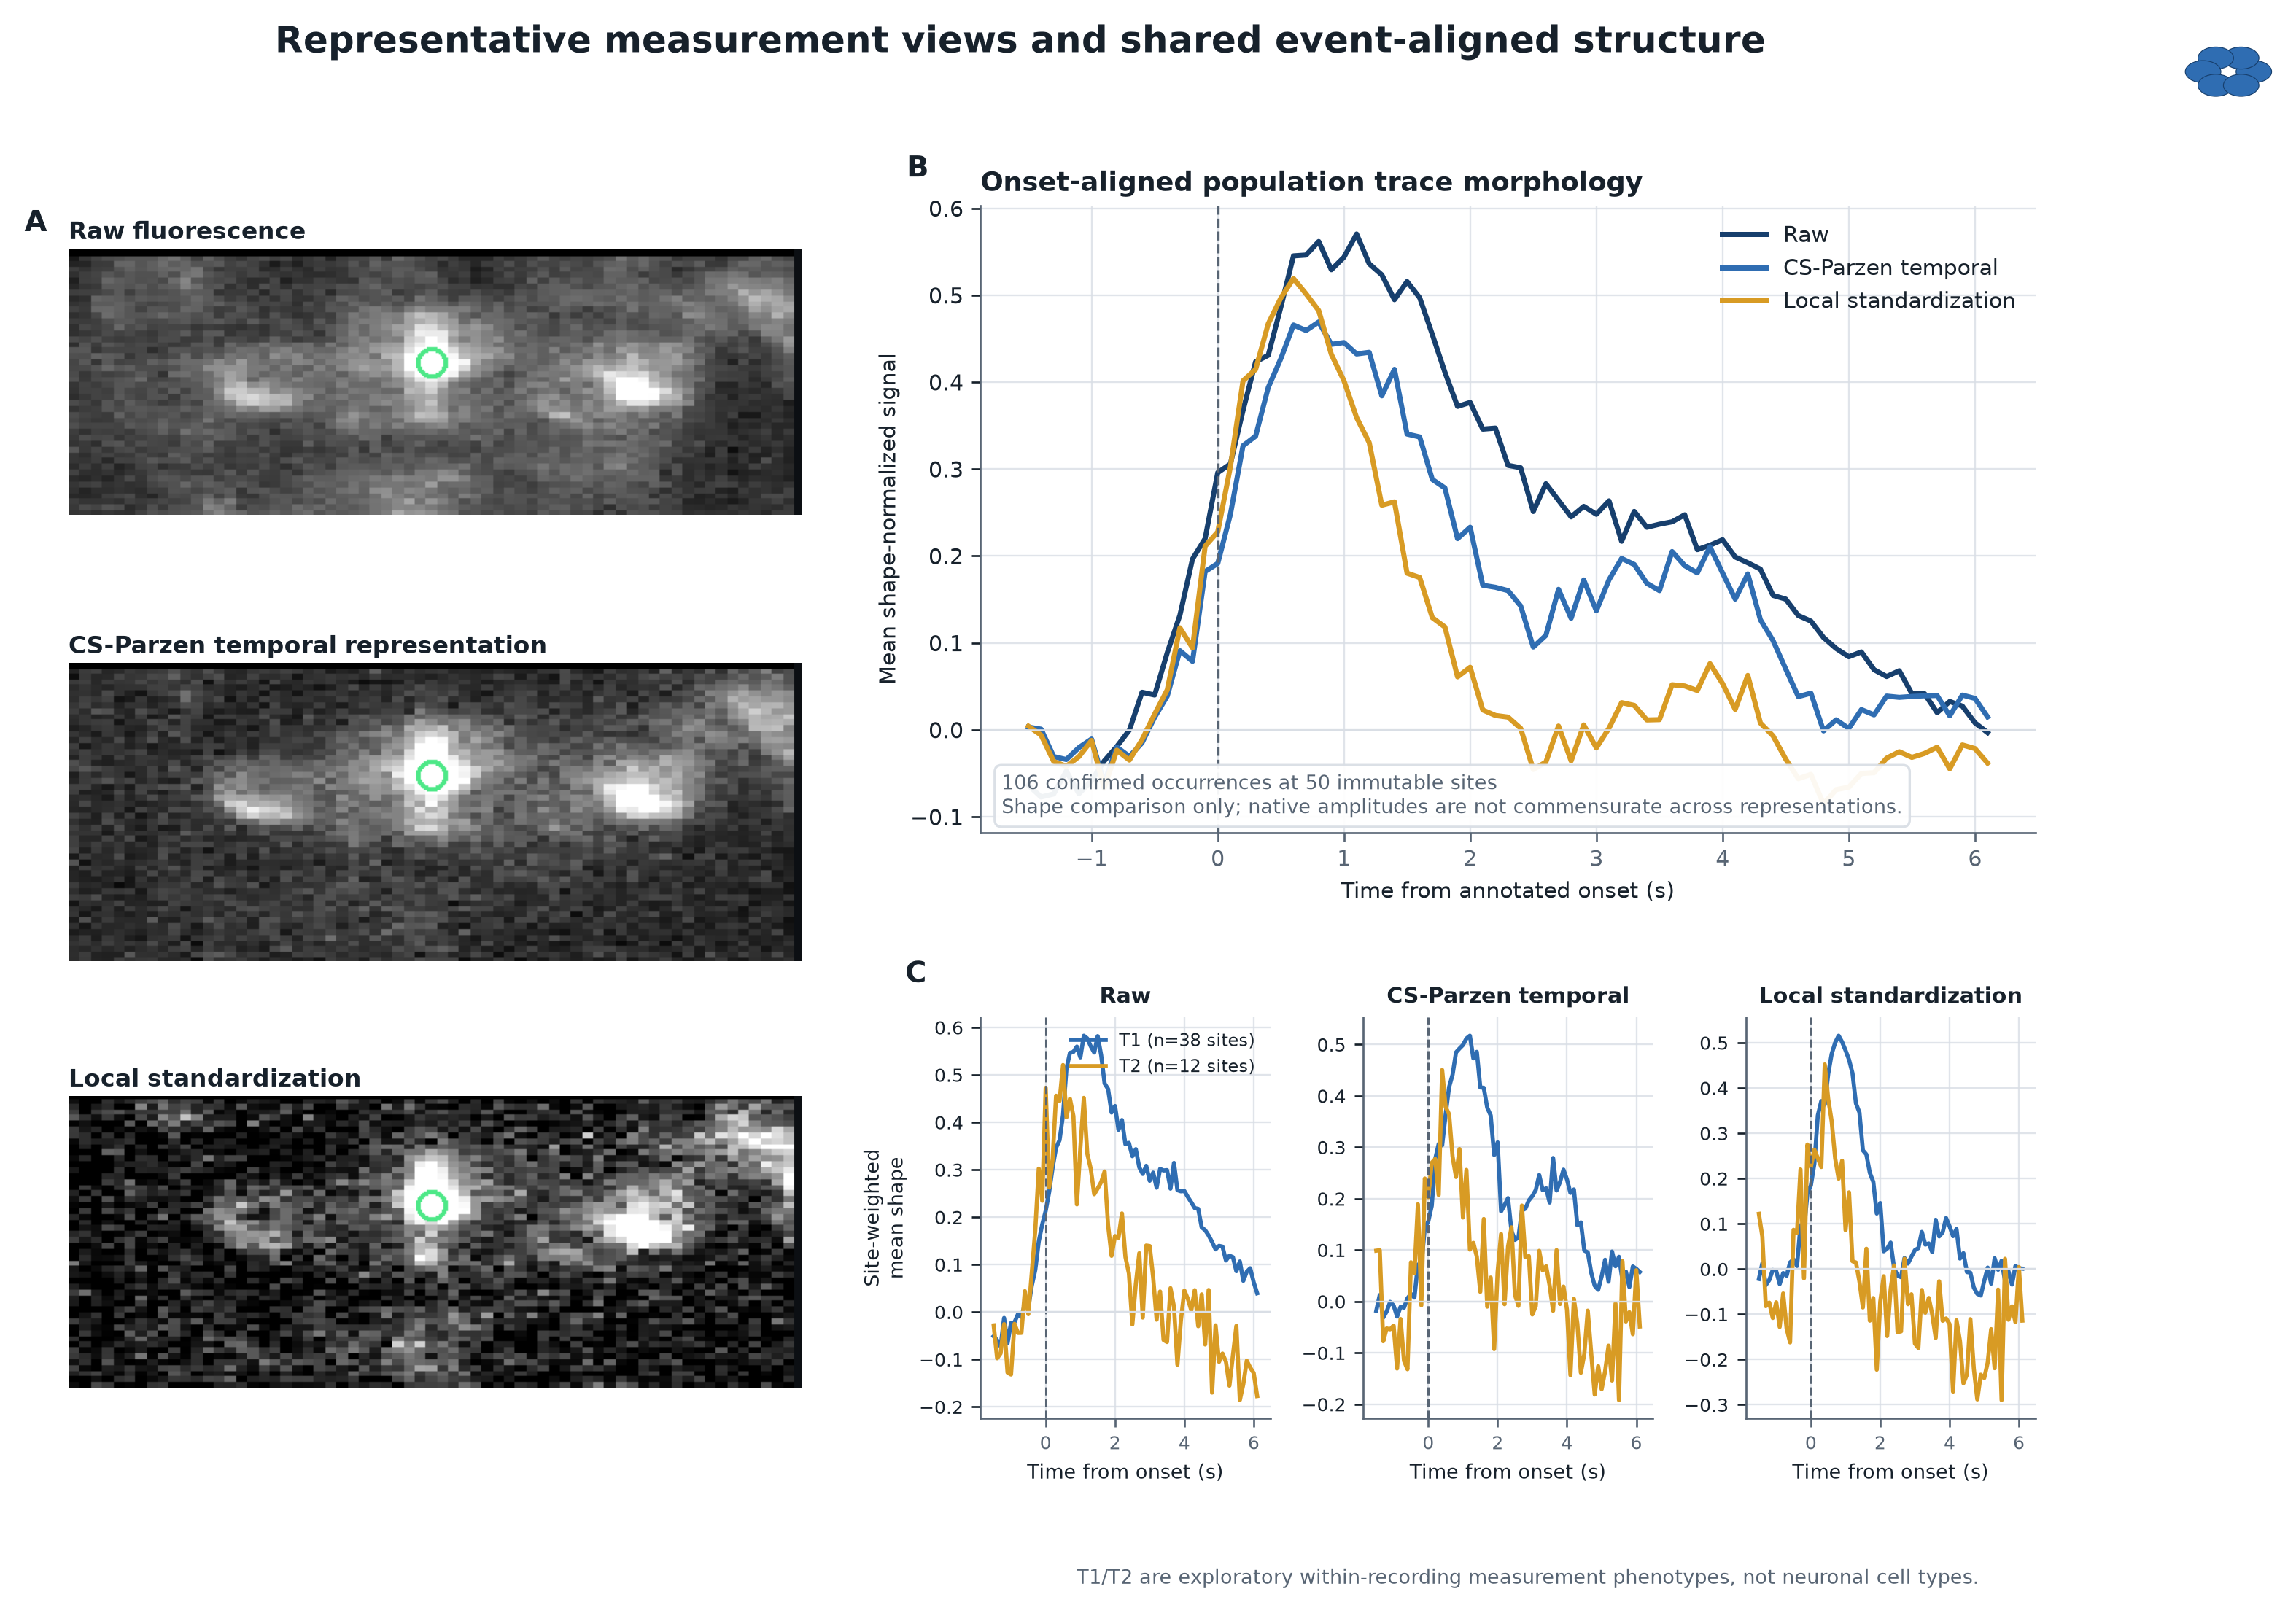
\includegraphics[width=\textwidth]{figures/venue/fig02_measurement_representations.png}
  \caption{Representative measurement views and shared event-aligned structure.
  The three image panels show stage-specific response-maximizing frames from one
  frozen representative occurrence; they are not same-frame images. The
  population curves summarize shape-normalized onset-aligned signals across
  \VenueCohortOccurrences{} occurrences at \VenueCohortSites{} sites. Panel C
  shows site-weighted mean shapes for the exploratory T1
  (\VenueTraceClassOneSites{} sites) and T2
  (\VenueTraceClassTwoSites{} sites) measurement phenotypes. Native amplitudes
  are not compared across representations, the phenotypes are not neuronal cell
  types, and no transformed component is named as a neuron.}
  \label{fig:venue-representations}
\end{figure*}
